%!TEX root = ../Thesis.tex
\section{Functions of the International Monetary Fund}
\label{sec:functions}

\subsection{Economic Surveillance}
Economic surveillance of the individual member countries, called bilateral surveillance and surveillance of the global economy, called multilateral surveillance is important for identifying possible stability and growth risks before a country is affected by them and is then in need of support. In our globally connected world, problems of one country can severely affect many other countries. Members of the \gls{IMF} get visited by \gls{IMF} staff once a year, where they hold discussions with government officials, central bank officials, labor unions and other important stakeholders of the country’s economy. These discussions focus on e.g.: exchange rates; monetary, fiscal and regulatory policies and critical structural reforms. The \gls{IMF} staff conducting these discussions then report to the Executive Board, which is comprised 24 directors, who are elected by the member countries or by groups of member countries - the director for Germany is Ruediger Wilhelm von Kleist for example. The executive board is also responsible for any changes of funding restrictions and any other change in the \gls{IMF}. Another aspect of economic surveillance is the global oversight, where the \gls{IMF} monitors and analyzes regional and global economic trends, which results in a monthly report, called the \enquote{World Economic Outlook}. In this report, which is commonly over 200 pages long, the \gls{IMF} highlight changes in economies around the world. Changes in global imports or unit labor cost and compensation for example.

\begin{figure}[!ht]
\centering
\begin{minipage}[t]{.7\textwidth} % Breite, z.B. 1\textwidth		
\caption{Unit Labor Cost and Compensation} % Überschrift
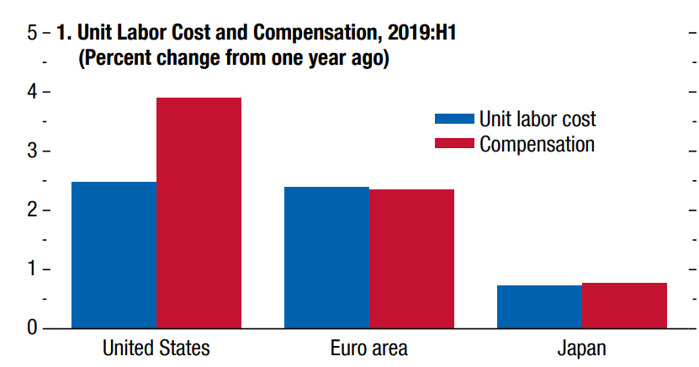
\includegraphics[width=1\textwidth]{img/laborcostcompensation.png}\\ % Pfad
\source{https://www.imf.org/en/Publications/WEO/Issues/2019/10/01/world-economic-outlook-october-2019} % Quelle
\label{fig:weoexample1}
\end{minipage}
\end{figure}

\begin{figure}[!ht]
\centering
\begin{minipage}[t]{.7\textwidth} % Breite, z.B. 1\textwidth		
\caption{Contribution to Global Imports} % Überschrift
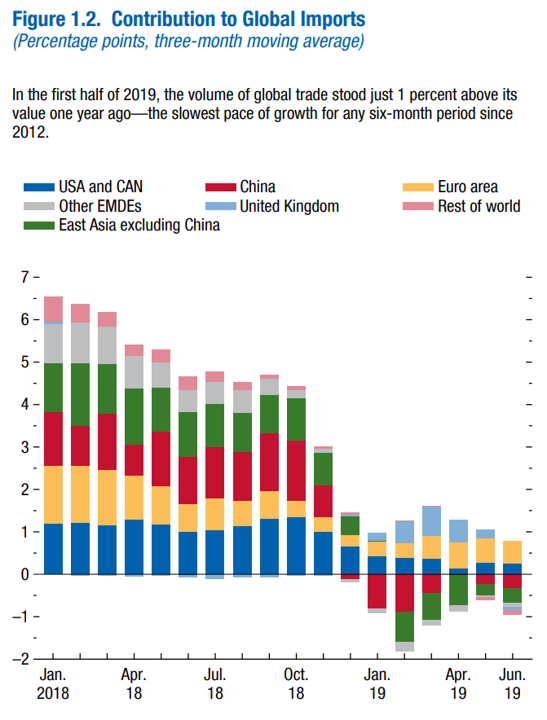
\includegraphics[width=1\textwidth]{img/globalimports.png}\\ % Pfad
\source{https://www.imf.org/en/Publications/WEO/Issues/2019/10/01/world-economic-outlook-october-2019} % Quelle
\label{fig:weoexample2}
\end{minipage}
\end{figure}

\subsection{Financial Assistance}
The most well-known function of the \gls{IMF} is their financial assistance of \enquote{countries hit by crises by providing them financial support to create breathing room as they implement adjustment policies to restore economic stability and growth.}\cite{InternationalMonetaryFundIMFLending2020}
The \gls{IMF} has its own currency called \gls{SDR}. It gets determined daily adjusting for the countries’ currencies change of value. As of March 29, 2020, for each Euro you get about 0.8 \gls{SDR}s or for each U.K. pound you get about 0.89 \gls{SDR}s.\cite{InternationalMonetaryFundSDRsper2020} Originally a \gls{SDR} was defined as the equivalent of 0.888671 grams of fine gold – which was exactly US\$1 at the time.\cite{InternationalMonetaryFundSpecialDrawing2020} Currently, the \gls{IMF} has a reserve of about US\$1 trillion available for lending to its member countries.\cite{InternationalMonetaryFundTheIMF2019} This reserve is made up of the so called \enquote{IMF Quota Subscription} each country has to pay upon joining the \gls{IMF}. The quota is also the reference of amount of votes the country has in the Executive Board and the amount a country can lend is also based on that quota – it gets calculated by adding up 50\% of the countries’ GDP, 30\% of its economic openness, 15\% of the economic variability and 5\% of its foreign country currency reserves, corrected with a compression factor, currently about 0.95 to make all its member countries comparable. For example, the quotas of Germany, the UK and the US are as follows: Germany: 26,635.4 million \gls{SDR}, UK: 20,155.1 million \gls{SDR}, US: 82,994.2 million \gls{SDR}.\cite{InternationalMonetaryFundIMFMembers2020} Currently, the \gls{IMF} has lending arrangements in 36 countries, most of which are either \enquote{\gls{EFF}} or \enquote{\gls{ECF}}.\cite{InternationalMonetaryFundIMFLending2020b} 
But why do crises occur? – Crises can occur because of domestic factors, like inappropriate fiscal and money policies; an exchange rate fixed at an inappropriate level or a weak financial system, but they can also occur because of external factors, like shocks from natural disasters – like the Corona virus outbreak currently. Especially low-income countries are affected by external factors, because they don’t have the financial power to prepare for such disasters. Lending money at below open market interest rates help countries in need in giving them time to implement adjustments to their economy to get financially stable again. For example, when prices of exported goods suddenly drop, the \gls{IMF} can loan the country money to implement measures to strengthen the economy and widen the country’s range of export goods. 
To apply for a loan you simply apply for it at the \gls{IMF}, then \gls{IMF} staff meets with the government and assesses the economic and financial situation of the country, then the \gls{IMF} staff determines the size of the country’s financial need and determines a policy program the country in need has to agree on and implement during the lending arrangement in order to receive the funding. The country in need then must write a “Letter of Intent” and “Memorandum of Understanding” and present them to the Executive Board, which then decided whether and if, what type of lending arrangement the country gets.\cite{InternationalMonetaryFundIMFLending2020}
The \gls{IMF} has different types of lending arrangements to fit different circumstances, they all mainly differ by who is eligible for the arrangement and how long the arrangement can maximally last – the current lending arrangements are as follows:
\glsreset{ECF} 
\glsreset{EFF} 
\begin{compactitem}
	\item \gls{SBA}: 3 countries in active arrangement, duration of up to 36 months.
	\item \gls{EFF}: 15 countries in active arrangement, duration of up to 10 years
	\item \gls{FCL}: 2 countries in active arrangement, duration of up to 5 years
	\item \gls{PLL}: Morocco currently in active arrangement, only countries with sound policies can apply for this arrangement, duration of up to 2 years
	\item \gls{PRGT}: support for low-income countries
	\item \gls{SCF}: Honduras currently in active arrangement, only countries eligible for the \gls{PRGT} are eligible, duration of up to 36 months
	\item \gls{ECF}: Honduras currently in active arrangement, only countries eligible for the \gls{PRGT} are eligible, duration of up to 5 years
	\item \gls{RCF}: no country currently in active arrangement, only countries eligible for the \gls{PRGT} are eligible, duration of up to 10 years
\end{compactitem}
In the EFF a country can normally borrow up to 145\% of the country’s \gls{IMF} quota annually and 435\% of the \gls{IMF} quota cumulative. There also is a commitment fee for each amount withdrawn from the fund, for example 30 basis points of the quota for a lending amount between 115\% and 575\%. The interest rate is the current \gls{SDR} interest rate plus 100 basis points (which is 1\%). Then there also is a service charge of 50 basis points of each amount drawn.
A country can apply for the \gls{ECF} if the purpose of funding is to support the country’s economic programs towards a more stable and sustainable economic position. Eligible are only countries, which also are eligible for the \gls{PRGT} and face a protracted balance of payments problem. Initially the country can apply for 3 to 4 years of aid, but only for a maximum of 5 years in whole. Whether a country gets access to funding via this arrangement is decided on a case-by-case basis and the funding is limited to 75\% of the quota per year and a total of 225\% of the quota.


\subsection{Capacity Development}